\documentclass{beamer}
\usepackage[orientation=portrait,size=a0,scale=1.4,debug]{beamerposter}
\mode<presentation>{\usetheme{ZH}}
\usepackage{chemformula}
\usepackage[utf8]{inputenc}
\usepackage[english]{babel} % required for rendering German special characters
\usepackage{siunitx} %pretty measurement unit rendering
\usepackage{hyperref} %enable hyperlink for urls
\usepackage{ragged2e}
\usepackage[font=scriptsize,justification=justified]{caption}
\usepackage{array,booktabs,tabularx}
\usepackage[ruled,noend,linesnumbered]{algorithm2e}
\usepackage{bm}

\newcolumntype{Z}{>{\centering\arraybackslash}X} % centered tabularx columns
%\sisetup{per=frac,fraction=sfrac}

\title{\huge Zero-shot Crate Digging $\rightarrow$ DJ Tool retrieval using Speech Activity, Music Structure and CLAP embeddings}
\author{Iroro Orife}
\institute[ETH]{Independent}
\date{\today}

% edit this depending on how tall your header is. We should make this scaling automatic :-/
\newlength{\columnheight}
\setlength{\columnheight}{104cm}

\begin{document}
\begin{frame}
\begin{columns}
	\begin{column}{.43\textwidth}
		\begin{beamercolorbox}[center]{postercolumn}
			\begin{minipage}{.98\textwidth}  % tweaks the width, makes a new \textwidth
				\parbox[t][\columnheight]{\textwidth}{ % must be some better way to set the the height, width and textwidth simultaneously
				
				
				     % TOP LEFT SECTION
					\begin{myblock}{What are DJ Tools?}
					In genres like Hip-Hop, RnB, Reggae, Dancehall and every Electronic/Dance/Club style, DJ tools are a special set of audio files of short, simplified musical phrases retrieved, curated from existing music, or composted specifically to heighten the DJ's musical performance and creative mixing choices.
						
						\vspace{0.7em}

						\begin{itemize}
							\item Acapella loops, vocal chants, spoken word, one shot vocal samples
							\item Purely instrumental (no drums) piano, guitar, strings, horns 
							\item Drum loops, solo percussion, drum breaks
							\item Sound effects: risers, sweeps, sirens, vinyl fx, 
							\item Scratch and Battle loops

						\end{itemize}
						\vspace{0.7em}

						\begin{figure}
							\begin{minipage}{0.43\textwidth}
								\centering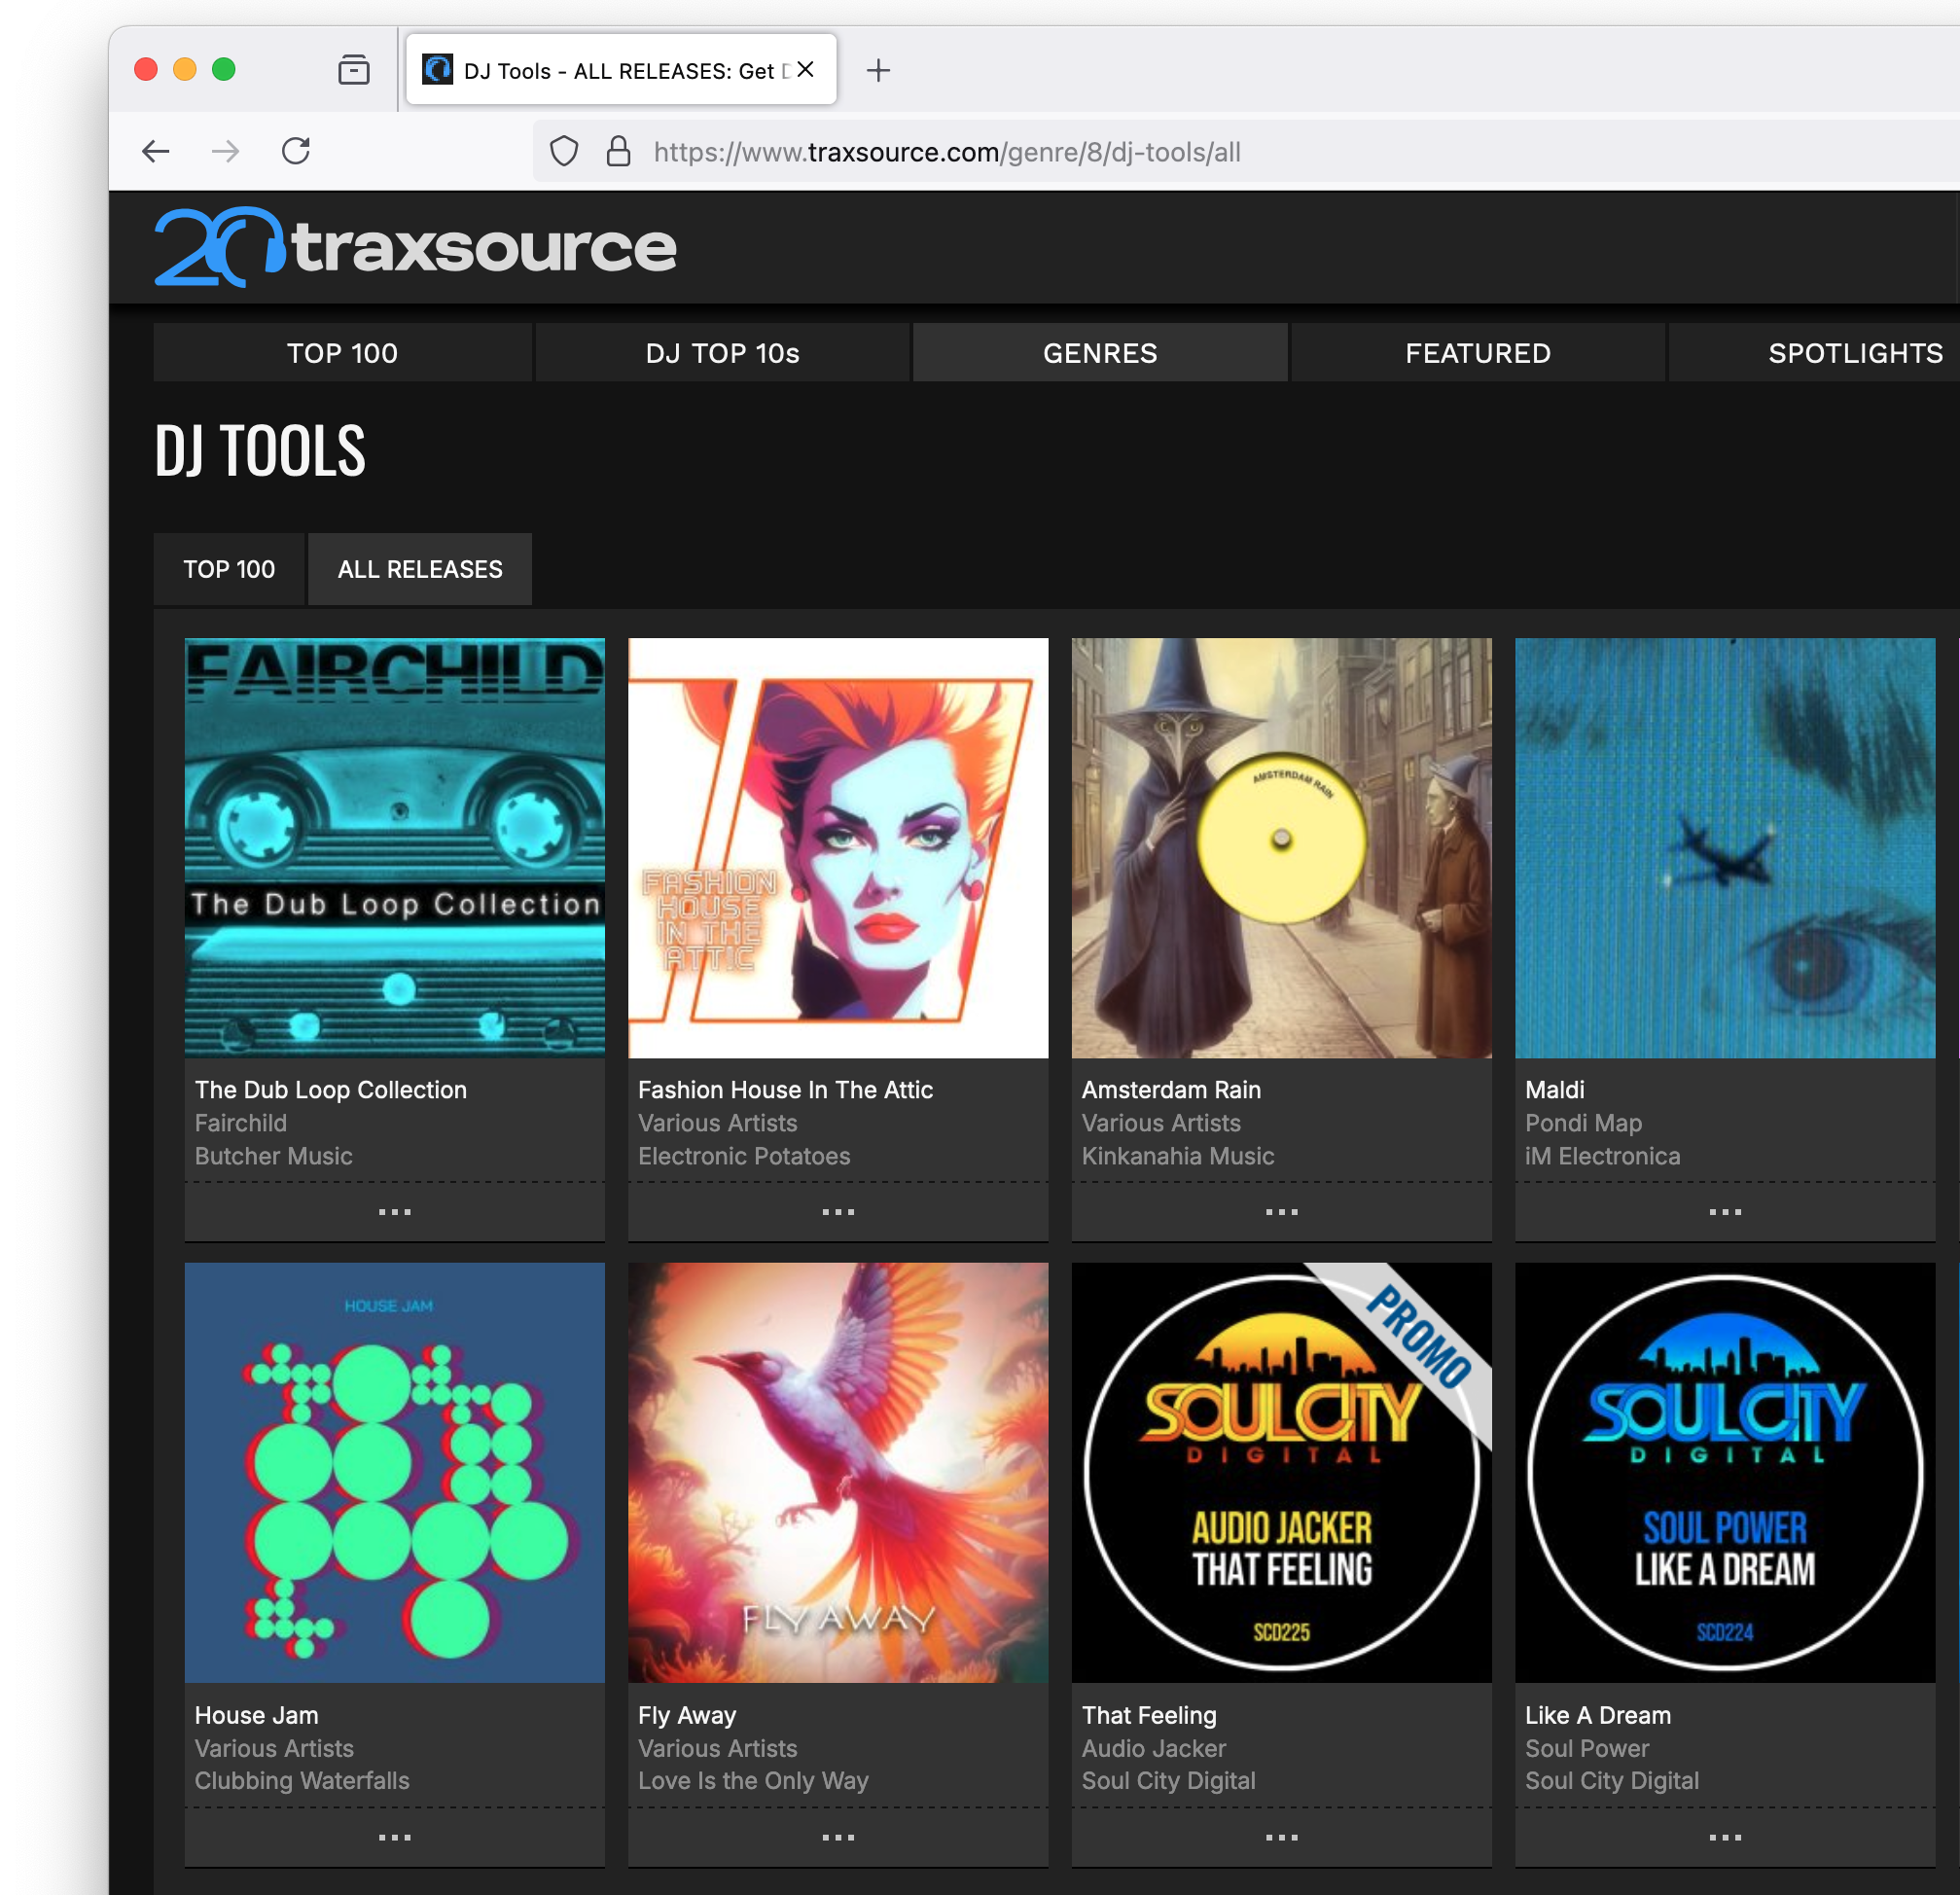
\includegraphics[width=0.8\textwidth]{img/traxsource_djtools.png}
								\caption{Traxsource DJ Tools shop}
							\end{minipage}
						\end{figure}


			            \begin{figure}
			              \begin{minipage}{0.43\textwidth}
			                \centering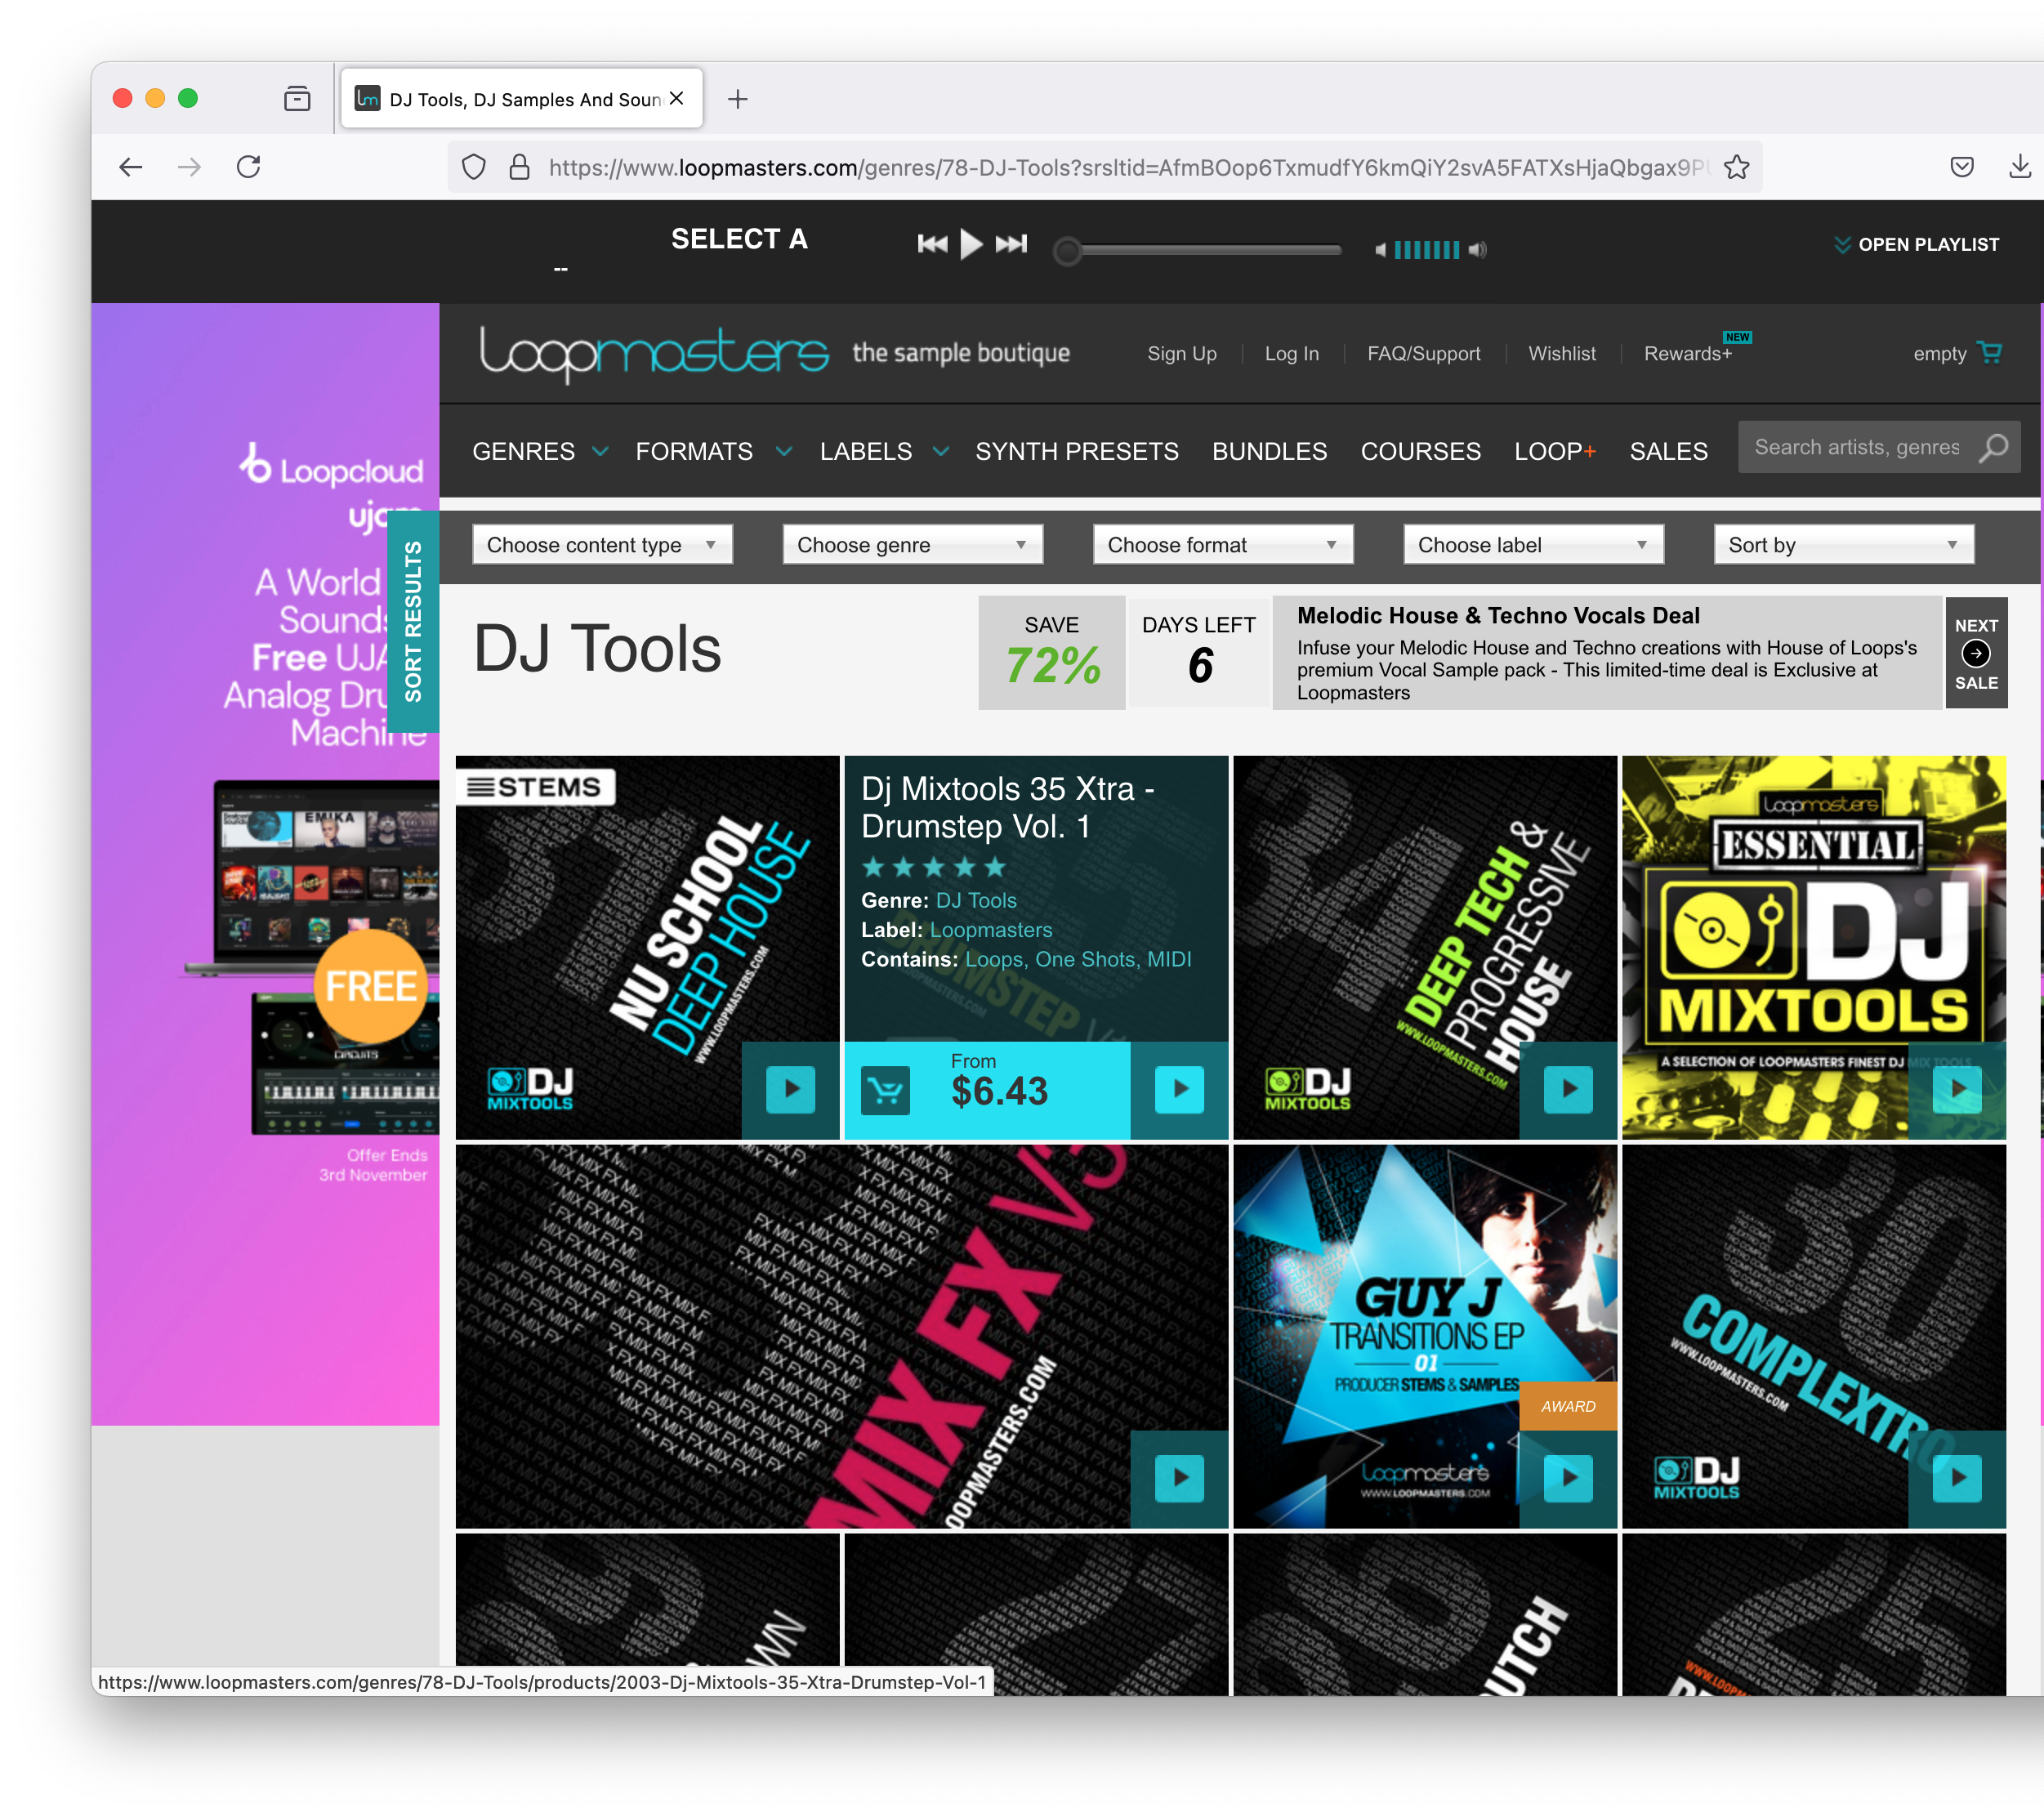
\includegraphics[width=0.85\textwidth]{img/loopmasters_djtools.png}
			                \caption{Loopmasters online shop. Note the specification of Loops, One-shots}
			              \end{minipage}
			              \hspace{1em}
			              \begin{minipage}{0.45\textwidth}
			                \centering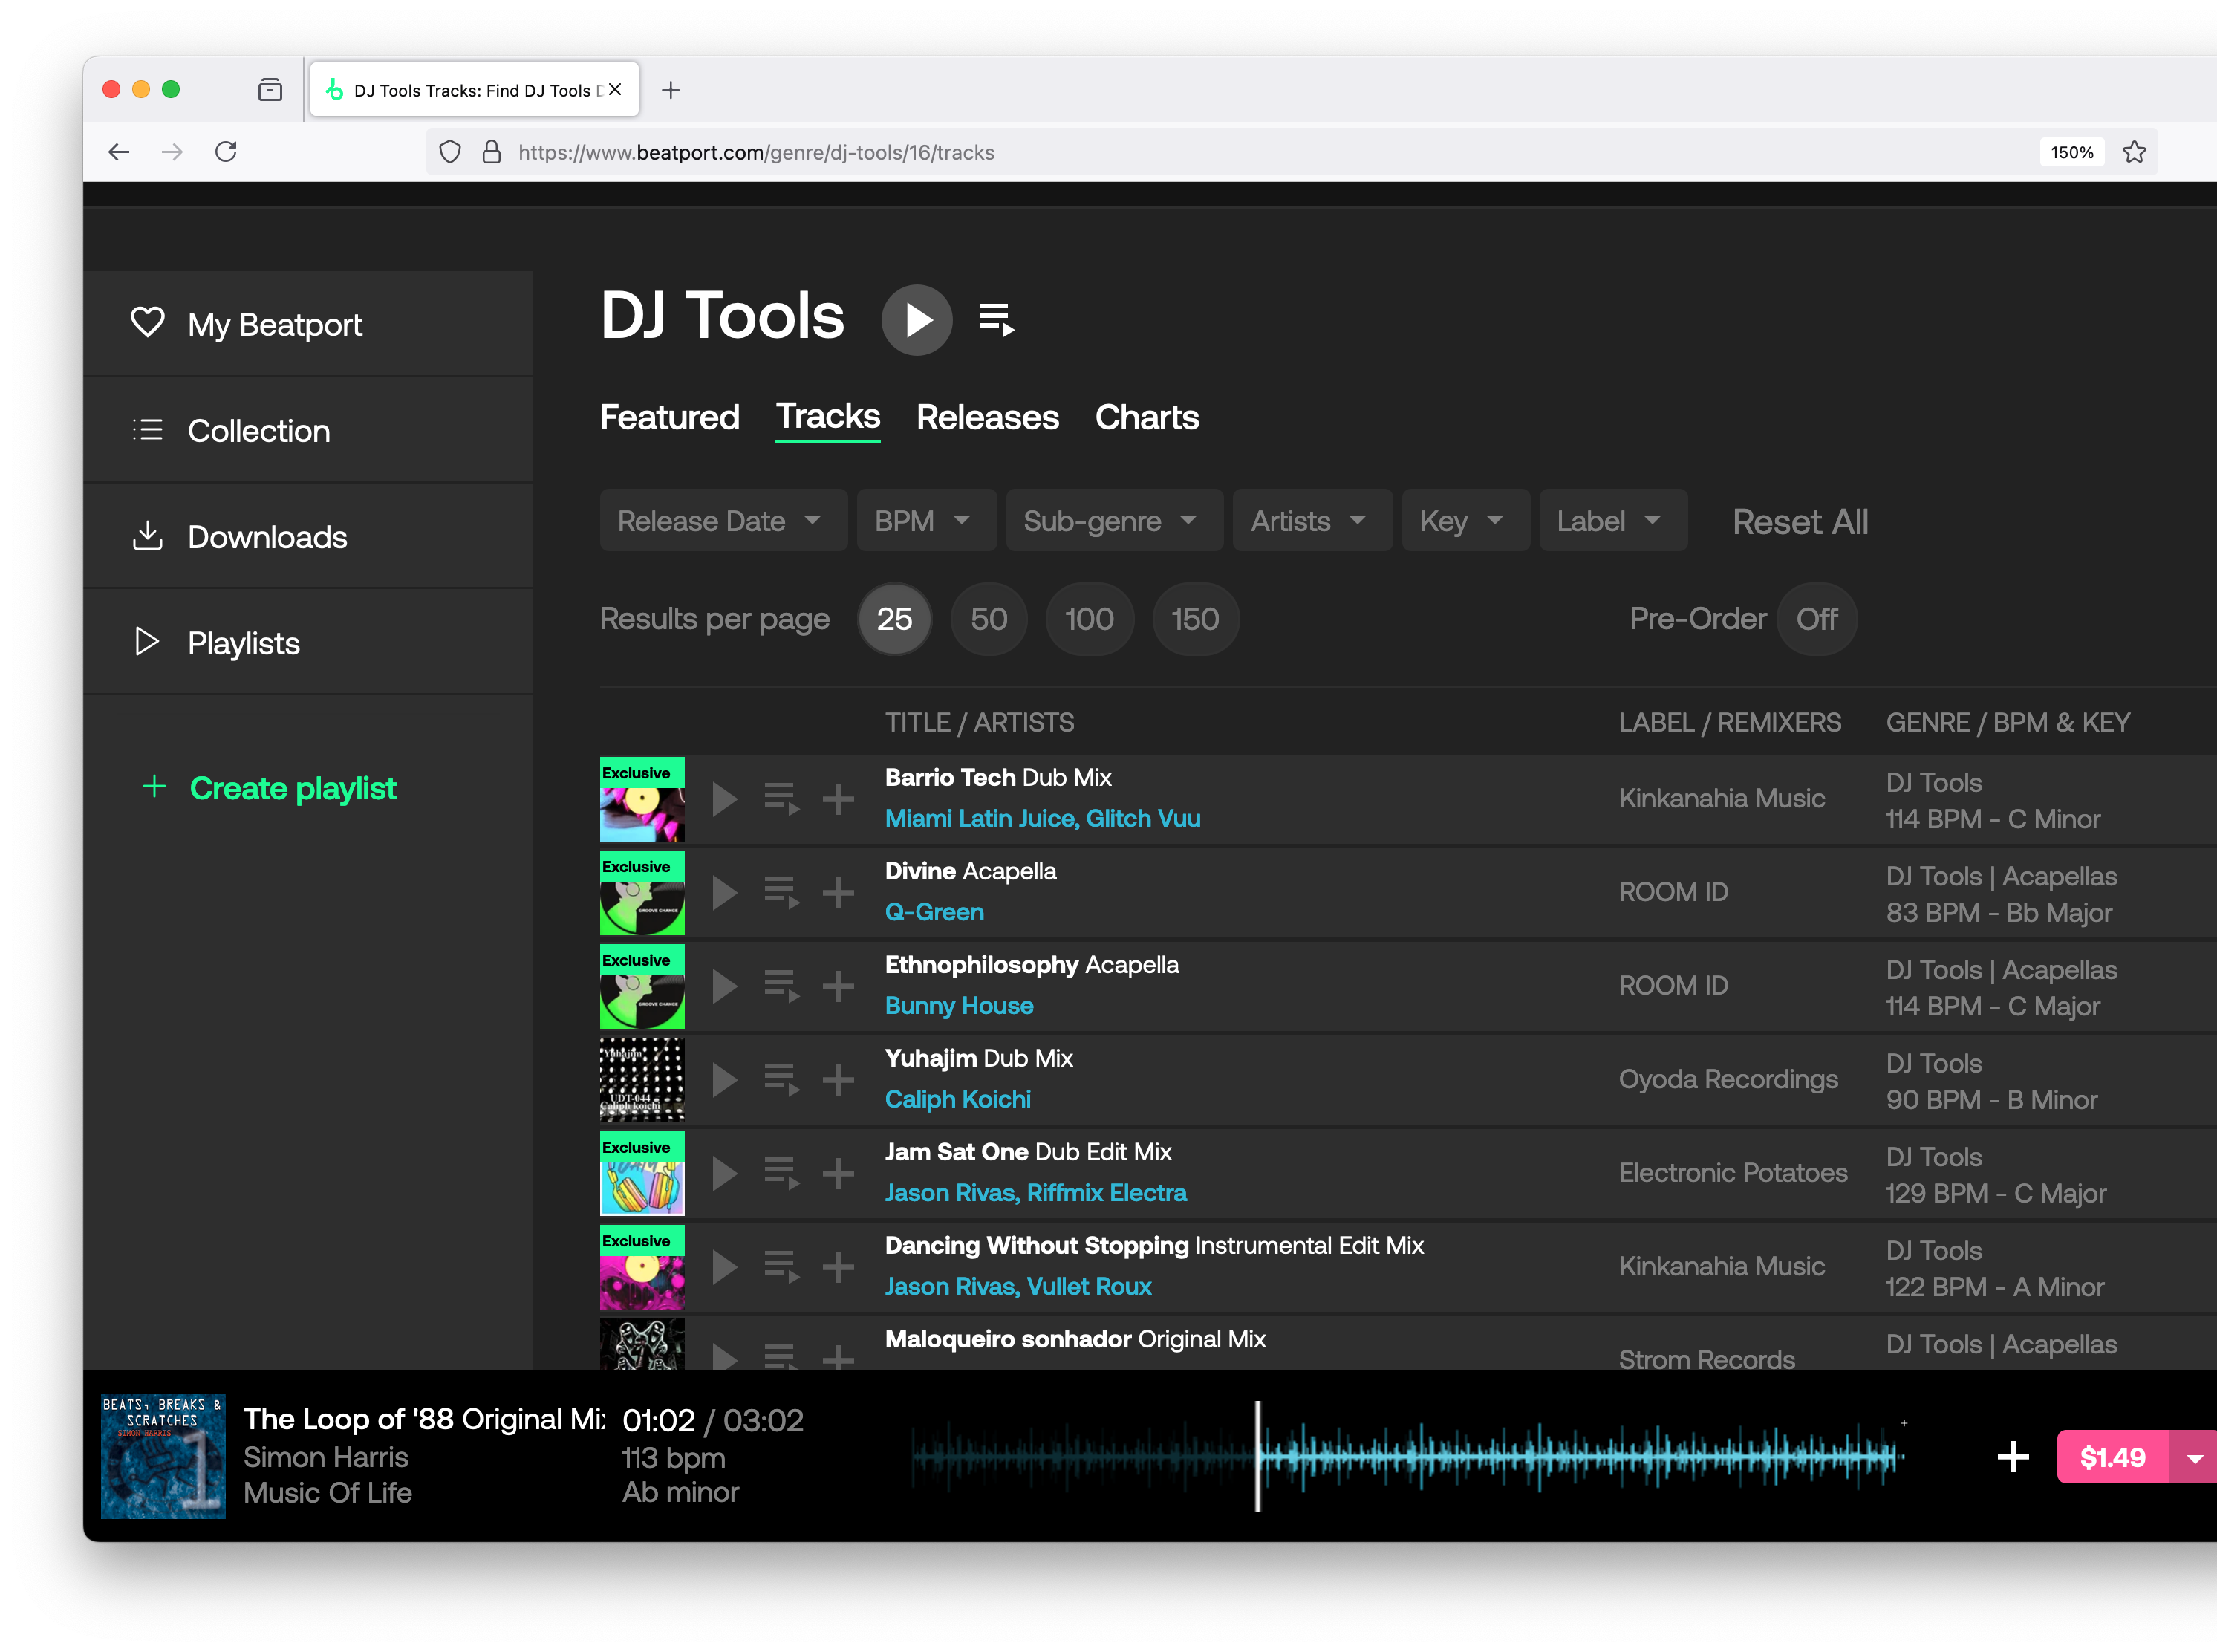
\includegraphics[width=1\textwidth]{img/beatport_djtools.png}
			                \caption{Beatport DJ Tools selection. Note the designated Genre, Key and BPM metadata}
			              \end{minipage}
			            \end{figure}
					\end{myblock}\vfill
					
%					BOTTOM LEFT SECTION
					\begin{myblock}{Software Demo Implementation}
					
					The DJ-tool classification system and its dependencies are fully open-source software (OSS) written in Python. Firstly, we run MSAF\footnote{https://github.com/urinieto/msaf} and SMAD\footnote{https://github.com/biboamy/TVSM-dataset/tree/master} to generate raw activities and structural boundaries, saved as CSV files \cite{Hung2022, nieto2016systematic}. Next, these are post-processed to yield lists of segment time ranges. Figure \ref{fig:msafsmadplot} shows the relationship between the boundaries and the speech activity for one song. 
					
					\vspace{1.2em}
					For zero-shot classification, we utilize the LAION version of CLAP\footnote{https://huggingface.co/laion/clap-htsat-unfused} hosted on Huggingface \cite{elizalde2022claplearningaudioconcepts, WuClap2023}. Finally, we manually create a list of descriptive text strings for each class, as listed in Table \ref{tab:djtool_texts}.
					\vspace{1.2em}

			 \begin{algorithm}[H]
			 \vspace{0.2em}
			    \caption{Zero-shot Crate Digging}\label{combo_algo}
			    	Create text prompts for $M$ classes \{$X^{t}_{1},...,X^{t}_{M}$\} \\
			    	 $\{E^{t}_{1},...,E^{t}_{M}\} \gets TextEncoder(\{X^{t}_{1},...,X^{t}_{M}\})$ \\
					\BlankLine
			        \For{song $s_i$ in the library $S_N$}{
			            $W^{s}, W^{m} \gets SMAD(s_i)$ \\ 
			            $B \gets MSAF(s_i)$  \\
			            Adjust boundaries $B_i$ to nearest $W^{s}$ \\
						Use $B$ to cut $s_i$ to audio files \{$X^a_1$,..., $X^a_N$\} \\
					    \BlankLine
			            \For{$j := $1 to $N$}{
			                $E^{a}_j \gets AudioEncoder(X^a_j)$ \\
			                $\vec{D} \gets Similarity(E^a_j, \{E^{t}_{1},...,E^{t}_{M}\})$ \\
			                $\vec{\bm{z}} \gets softmax(\vec{D})$ \\
			                Store predicted class, the $\mathop{\arg \max}$ of $\vec{\bm{z}}$\\
			                	\BlankLine
			               	\BlankLine
			            }
			        }
			 \end{algorithm}
			\vspace{0.4em}
		  \end{myblock}\vfill
		}\end{minipage}\end{beamercolorbox}
	\end{column}
	
	
	
	% TOP RIGHT SECTION
	\begin{column}{.57\textwidth}
		\begin{beamercolorbox}[center]{postercolumn}
			\begin{minipage}{.98\textwidth} % tweaks the width, makes a new \textwidth
				\parbox[t][\columnheight]{\textwidth}{ % must be some better way to set the the height, width and textwidth simultaneously
					\begin{myblock}{What is Zero-shot Audio Classification?}
%						\vspace{0.2em}
						\begin{figure}
							\begin{minipage}{.94\textwidth}
								\centering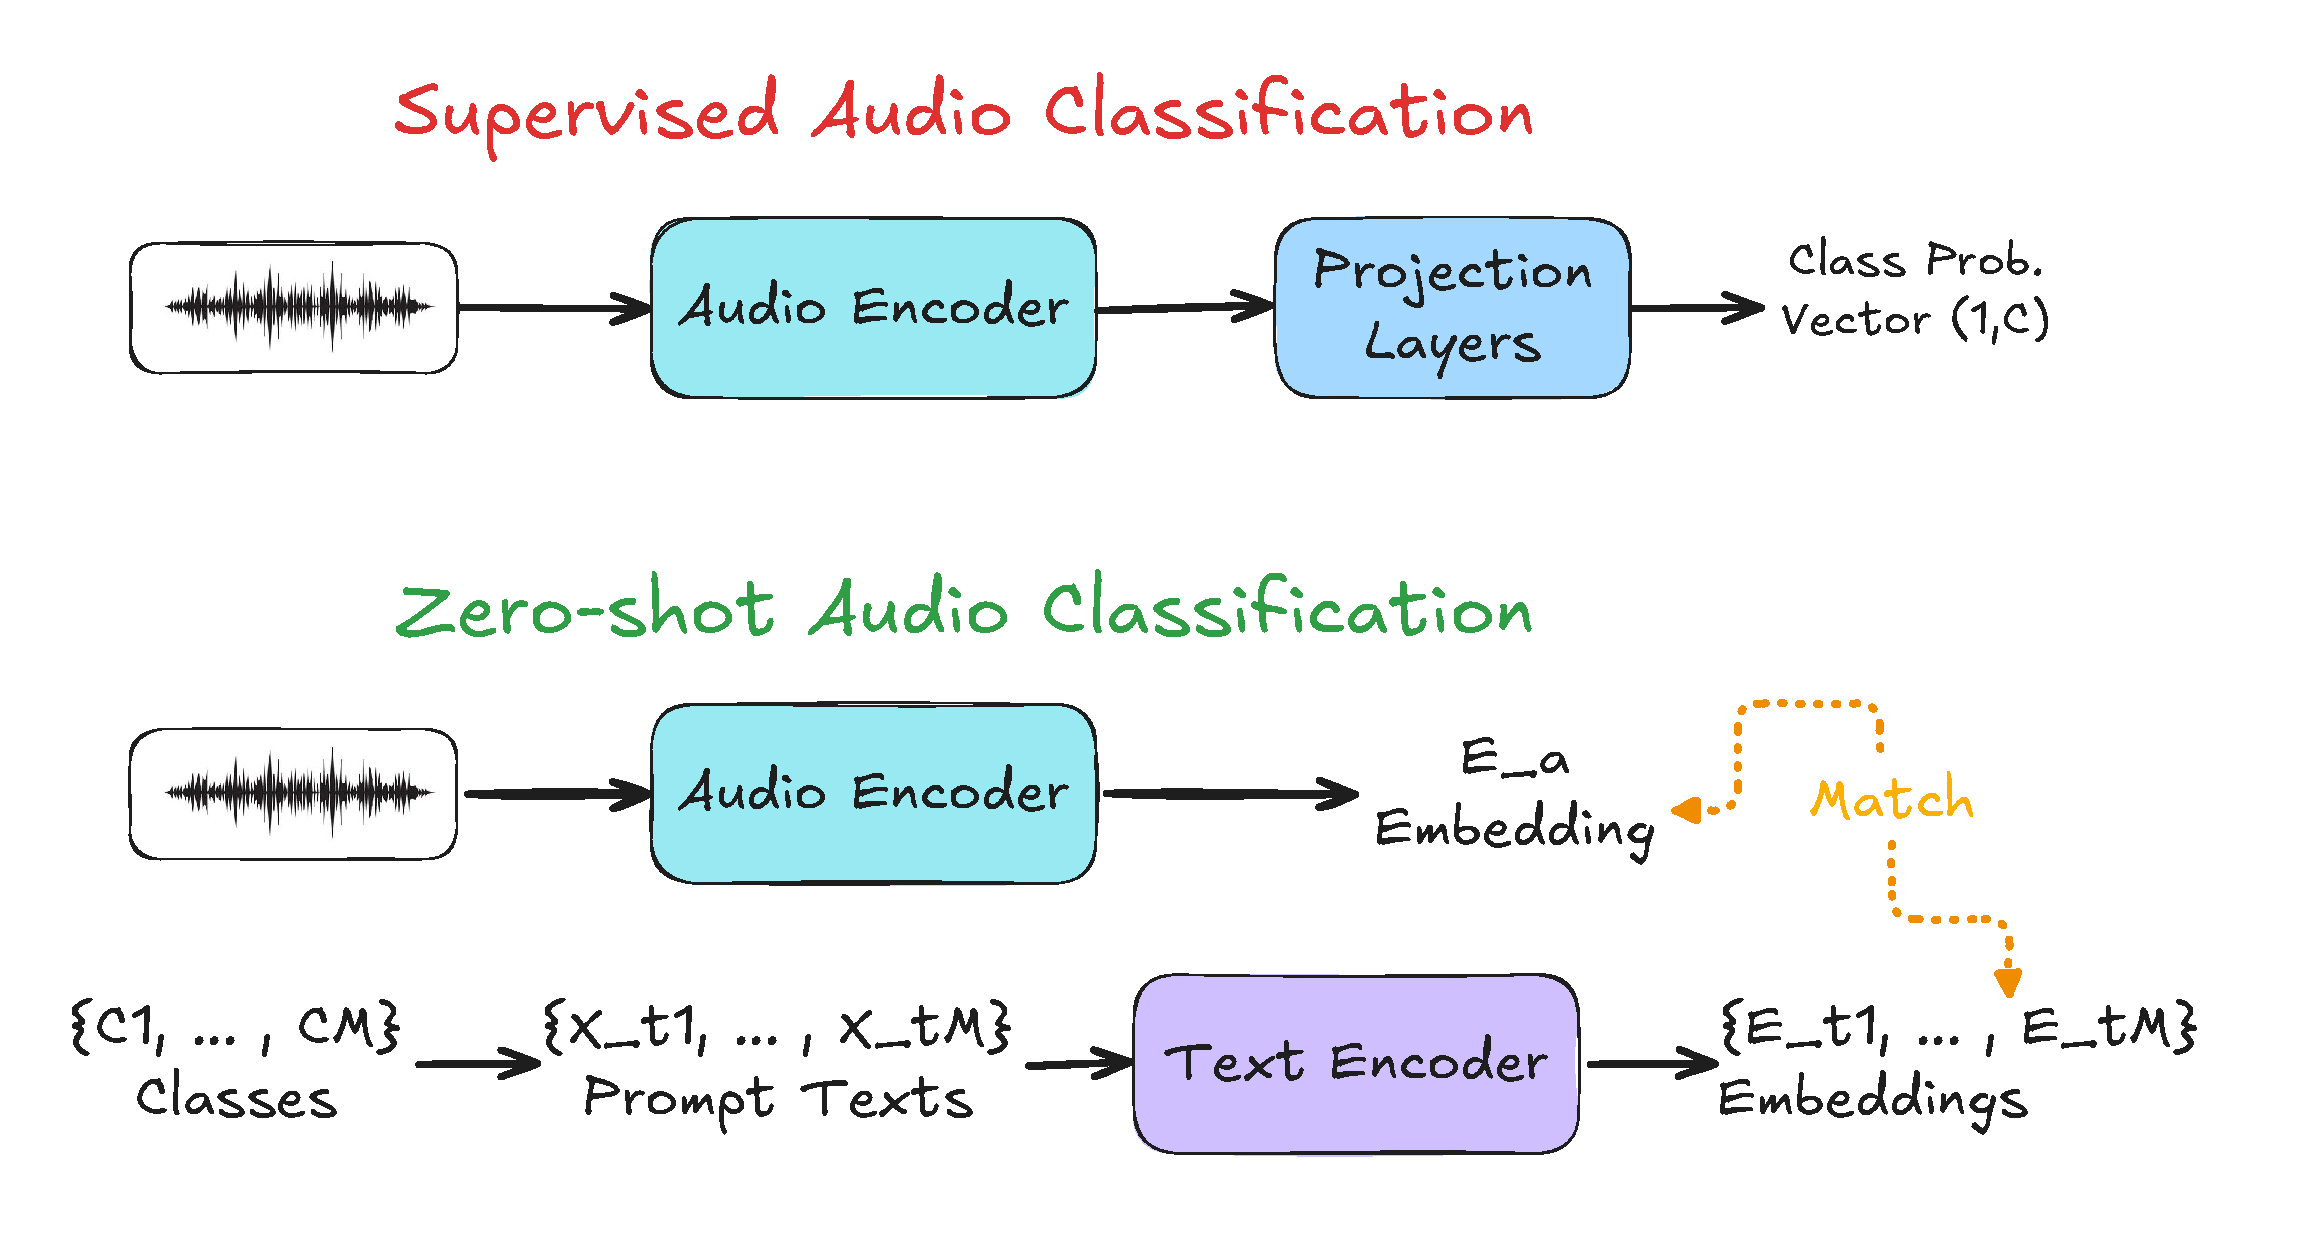
\includegraphics[width=\textwidth]{img/CLAP-ISMIR_lbd.pdf}
								\caption{}
							\end{minipage}
						\end{figure}
					\end{myblock}\vfill
					
					
			     % BOTTOM RIGHT SECTION
				\begin{myblock}{Speech Activity \& Music Structure Analysis}
			\vspace{1em}
			\begin{figure}
			 \centerline{
			 	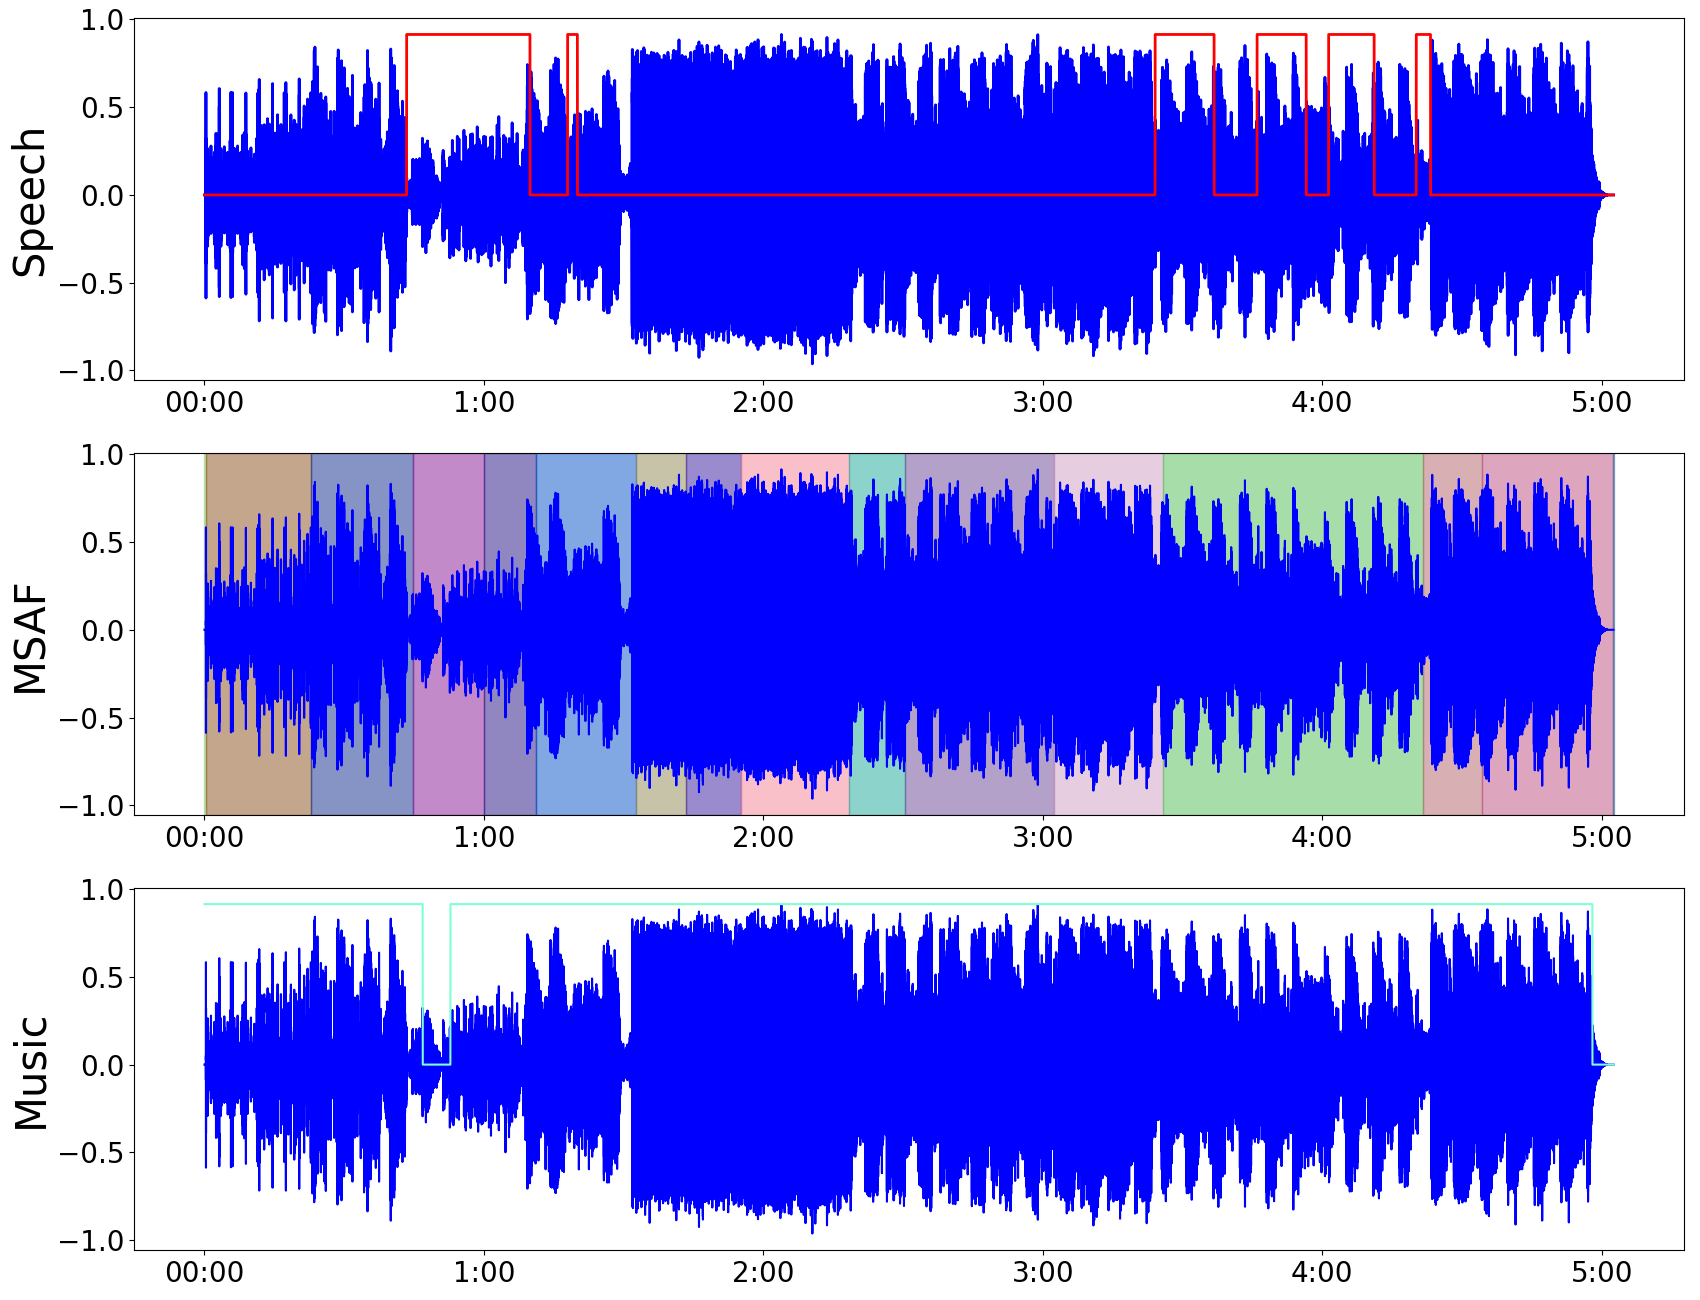
\includegraphics[alt={SMAD \& MSAF Analysis signals}, width=0.6\columnwidth]{img/smad_msaf.png}
			 	}
			 \caption{A 5 minute Ragga Jungle song overlaid with detected speech, \\ music activity and music-structural boundaries}
			 \label{fig:msafsmadplot}
			\end{figure}
	
%			\vspace{0.4em}
			
			\begin{table}
			 \begin{center}
			 \begin{tabular}{lc}
			  \midrule
			  \textbf{DJ Tool class} & \textbf{Example text description} \\
			  \midrule
				Acapella loops & ``acapella, expressively sung vocal tracks, purely acoustic''  \\
				Sound effects &  ``siren, riser sound effects, whoosh, crash, synthetic''\\
				Drums breaks  & ``drums, funky drummer, drum solo, Amen breakbeat''  \\
				Melodic hooks & ``strings, solo guitar, piano melodies, synths instrumental''  \\
				Battle tracks & ``vinyl scratch loop, turnatablist DJ battle sounds''   \\
			 \end{tabular}
			\end{center}
			 \caption{In practise, text descriptions are more tortuous}
			 \label{tab:djtool_texts}
			\end{table}
			
		\end{myblock}\vfill
					
					
					% BOTTOM RIGHT SECTION
					\begin{myblock}{Results: Making music with the system}

					We evaluated the system on 10+ albums from the author's DJ library $\rightarrow$ 

						\begin{itemize}
							\item Vocal and drums tool classes perform better than short, burstier sound effects 							
							\item Performance is sensitive to \textit{precise language}. Adding generic terms or entire genres (e.g. ``hip-hop, drum and bass'') to a class description led to markedly worse results overall
							\item For best results, the class descriptions should not overlap
							\item One challenge was to determine the optimal segmentation for CLAP classification, while slicing the song appropriately for use by DJs.
							\item Playing with the system and making music with the retreived DJ tools led to unexpectedly delightful mixing sessions
						\end{itemize}
	\end{myblock}\vfill
					
					
					\begin{myblock}{References}
						\footnotesize
						\bibliographystyle{abbrv}
						\bibliography{./bib}
					\end{myblock}\vfill
		}\end{minipage}\end{beamercolorbox}
	\end{column}
\end{columns}
\end{frame}
\end{document}
